\selectlanguage{english}%

\chapter{Modelagem}

\section{Modelo Não Linear}
Baseado nos princípios de conservação de massa e na lei de Bernoulli para líquidos incompressíveis tem-se o seguinte sistema de equações não lineares que descrevem o processo.

\begin{equation}
	\begin{cases}
		\dot{h_{1}} = \frac{1}{A_{1}}(a_{3}\sqrt{2gh_{3}} + \gamma_{1}k_{1}v_{1} - a_{1}\sqrt{2gh_{1}})\\
		
		\dot{h_{2}} = \frac{1}{A_{2}}(a_{4}\sqrt{2gh_{4}} + \gamma_{2}k_{2}v_{2} - a_{2}\sqrt{2gh_{2}})\\
		
		\dot{h_{3}} = \frac{1}{A_{3}}((1 - \gamma_{2})k_{2}v_{2} - a_{3}\sqrt{2gh_{3}})\\
		
		\dot{h_{4}} = \frac{1}{A_{4}}((1 - \gamma_{1})k_{1}v_{1} - a_{4}\sqrt{2gh_{4}})
	\end{cases}
\end{equation}
em que, $h_{i}$, $A_{i}$ e $a_{i}$ são o nível de água, a área da secção transversal e a área de secção transversal do orifício de saída do tanque i, $i=1,2,3,4$, respectivamente. A constante de fluxo e a tensão aplicada na bomba j são dadas respectivamente por $k_{j}$ e $v_{i}$, $j=1,2$. O parâmetro $\gamma_{1}$ é a razão entre os fluxos para os tanques 1 e 4, $\gamma_{2}$ é a razão entre os fluxos para os tanques 2 e 3 e g é a aceleração da gravidade. 

\section{Linearização}
Linearizando o sistema em torno dos ponto de operação $\overline{h}=(\overline{h_{1}},\overline{h_{2}},\overline{h_{3}},\overline{h_{4}})$ e $\overline{v}=(\overline{v_{1}},\overline{v_{2}})$, por expansão em série de Taylor, obtém-se a seguinte representação no espaço de estados:

\begin{multline}
	\begin{bmatrix}
		\dot{\Delta h_{1}} \\
		\dot{\Delta h_{2}} \\
		\dot{\Delta h_{3}} \\
		\dot{\Delta h_{4}} 
	\end{bmatrix}
	= 
	\begin{bmatrix}
		\frac{-a_{1}\sqrt{2g}}{2A_{1}\sqrt{h_{1}}} & 0 & \frac{a_{3}\sqrt{2g}}{2A_{1}\sqrt{h_{3}}} & 0 \\
		0 & \frac{-a_{2}\sqrt{2g}}{2A_{2}\sqrt{h_{2}}} & 0 & \frac{a_{4}\sqrt{2g}}{2A_{2}\sqrt{h_{4}}} \\
		0 & 0 & \frac{-a_{3}\sqrt{2g}}{2A_{3}\sqrt{h_{3}}} & 0 \\
		0 & 0 & 0 & \frac{-a_{4}\sqrt{2g}}{2A_{4}\sqrt{h_{4}}}
	\end{bmatrix}
	\begin{bmatrix}
		\Delta h_{1} \\
		\Delta h_{2} \\
		\Delta h_{3} \\
		\Delta h_{4} 
	\end{bmatrix}
	+
	\begin{bmatrix}
		\frac{\gamma_{1}k_{1}}{A_{1}} & 0 \\
		0 & \frac{\gamma_{2}k_{2}}{A_{2}} \\
		0 & \frac{(1-\gamma_{2}) k_{2}}{A_{3}} \\
		\frac{(1-\gamma_{1})k_{1}}{A_{4}} & 0
	\end{bmatrix}
	\begin{bmatrix}
		\Delta v_{1} \\
		\Delta v_{2}
	\end{bmatrix}
	\label{eq2}
\end{multline}
\begin{equation}
	\begin{bmatrix}
		y_{1} \\
		y_{2} \\
		y_{3} \\
		y_{4} 
	\end{bmatrix}
	= 
	I
	\begin{bmatrix}
		\Delta h_{1} \\
		\Delta h_{2} \\
		\Delta h_{3} \\
		\Delta h_{4} 
	\end{bmatrix}
	\label{eq3}
\end{equation}

em que $y_{i}$ são as saídas medidas do sistema, $\Delta h_{i}=h_{i} - \overline{h_{i}}$, $\Delta v_{i}=v_{i} - \overline{v_{i}}$, e $i=1,2,3,4$.

E por fim, a matriz função de transferência do sistema obtida é:
\begin{equation}
	G(s) = 
	\begin{bmatrix}
		\frac{T_{1}\gamma_{1}k_{1}}{A_{1}(1+sT_{1})} &  \frac{T_{1}(1-\gamma_{2})k_{2}}{A_{1}(1+sT_{3})(1+sT_{1})} \\
		\frac{T_{2}(1-\gamma_{1})k_{1}}{A_{2}(1+sT_{4})(1+sT_{2})} &  \frac{T_{2}\gamma_{2}k_{2}}{A_{2}(1+sT_{2})} \\
		0 &  \frac{T_{3}(1-\gamma_{2})k_{2}}{A_{3}(1+sT_{3})} \\
		\frac{T_{4}(1-\gamma_{1})k_{1}}{A_{4}(1+sT_{4})} &  0 
	\end{bmatrix} 
	\label{eq4}
\end{equation}

em que $G(s)=\frac{\Delta h(s)}{\Delta v(s)}$ e $T_{i}=\frac{2A_{i}\sqrt{h_{i}}}{a_{i}\sqrt{2g}}$, $i=1,2,3,4$.

\section{Modelagem Fuzzy Takagi-Sugeno} \label{secModFuzzy}
\subsection{Variáveis Linguísticas}
	As linearizações do sistema são baseadas nos estados de em que os níveis do sistema são  estacionários, ou seja $\dot{h}(t) = 0$. Assim, o modelo linear, que trata o valor de desvio das variáveis, é dado por: 
		\begin{equation}
			\dot{h}(t) =  A \Delta h(t) +  B \Delta u(t)
		\end{equation}

	As variáveis aferidas da planta são os níveis, por este motivo serão as variáveis linguísticas definidas para o modelo fuzzy. Escolhem-se então "Nível do Tanque 1" e "Nível do Tanque 2" e os valores fuzzy {nível baixo, nível alto} para cada uma.

\subsection{Regras Se-Então}
	A combinação simples dos conjuntos de valores linguísticos fornece as seguintes regras Se-Então:
	\begin{itemize}
		\centering
		\item Regra 1: Se $h_1$ é baixo e $h_2$ é baixo, então $\dot{h}(t) =  A_1 \Delta h_1(t) +  B_1 \Delta u_1(t)$
		\item Regra 2: Se $h_1$ é baixo e $h_2$ é alto, então $\dot{h}(t) =  A_2 \Delta h_2(t) +  B_2 \Delta u_2(t)$
		\item Regra 3: Se $h_1$ é alto e $h_2$ é baixo, então $\dot{h}(t) =  A_3 \Delta h_3(t) +  B_3 \Delta u_3(t)$
		\item Regra 4: Se $h_1$ é alto e $h_2$ é alto, então $\dot{h}(t) =  A_4 \Delta h_4(t) +  B_4 \Delta u_4(t)$
	\end{itemize}

	Onde
	\begin{align}
		\Delta h_i(t) =
		\begin{bmatrix}
			h_1(t) - \bar{h_{1i}} \\
			h_2(t) - \bar{h_{2i}} \\
			h_3(t) - \bar{h_{3i}} \\
			h_4(t) - \bar{h_{4i}}
		\end{bmatrix} 
		&&
		\Delta u_i(t) = 
		\begin{bmatrix}
			u_1(t) - \bar{u_{1i}} \\
			u_2(t) - \bar{u_{12}}
		\end{bmatrix}
	\end{align}	

\subsection{Pertinência}
	Fazendo-se:
	\begin{itemize}
		\centering
		\item $M_1(h_1(t))$: Grau de pertinência fuzzy de $h_1(t)$ ao conjunto "Nível H1 Baixo" 
		\item $M_2(h_1(t))$: Grau de pertinência fuzzy de $h_1(t)$ ao conjunto "Nível H1 Alto"
		\item $N_1(h_2(t))$: Grau de pertinência fuzzy de $h_2(t)$ ao conjunto "Nível H2 Baixo"
		\item $N_2(h_2(t))$: Grau de pertinência fuzzy de $h_2(t)$ ao conjunto "Nível H2 Alto"
	\end{itemize}	
	
\subsection{Ativação}
	O nível de ativação de cada uma das Regras é dado respectivamente por:
	\begin{equation}
	\begin{aligned}
		w_{1}(t) = M_1(h_1(t)) * N_1(h_2(t)) \\
		w_{2}(t) = M_1(h_1(t)) * N_2(h_2(t)) \\
		w_{3}(t) = M_2(h_1(t)) * N_1(h_2(t)) \\
		w_{4}(t) = M_2(h_1(t)) * N_2(h_2(t))
	\end{aligned}
	\label{eqGrauAtiv4T}
	\end{equation}
	
\subsection{Modelo Final}
	O método de Takagi-Sugeno fornece, finalmente:
	\begin{align}
		\dot{h}(t) = \frac{\sum_{i=1}^{4}  w_i(h(t))(A_i \Delta h_i(t) +  B_i \Delta u_i(t))}{\sum_{i=1}^{4} w_i(h(t))}
	\end{align}

\subsection{Controlador Fuzzy}
	O desenvolvimento do controlador para este modelo segue os mesmos passos: realiza-se a sintonização do ganho $K$ a ser utilizado para cada regra, o grau de ativação de cada ganho é obtido pelas mesmas equações \ref{eqGrauAtiv4T}. O ganho final a ser utilizado é dado por:
	
	\begin{align}
		K = \frac{\sum_{i=1}^{4}  w_i(h(t))K_i}{\sum_{i=1}^{4} w_i(h(t))}
	\end{align}
	
	\begin{figure}
		\begin{centering}
			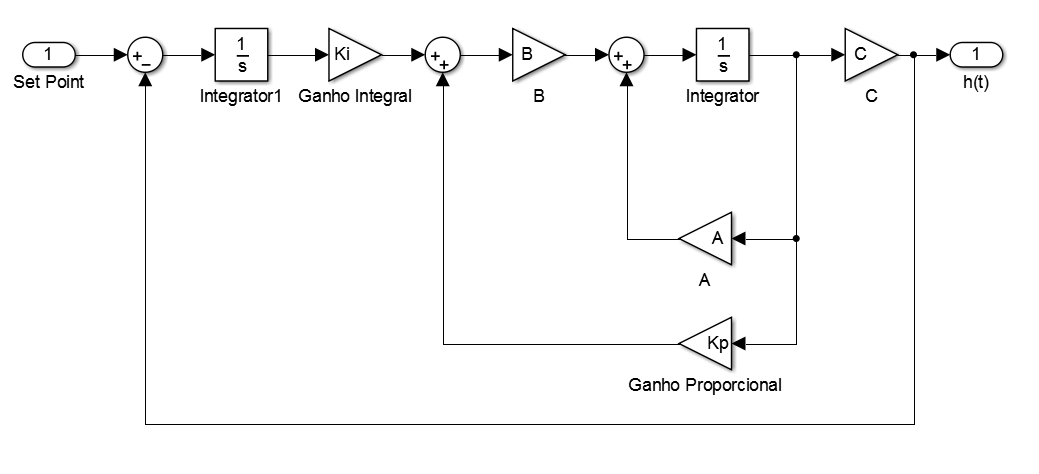
\includegraphics[width=\textwidth]{img/modelo_controlado.png}
			\par\end{centering}
		\caption{\label{figSimPlantCtrl}Espaço de estados da planta controlada}
	\end{figure}

\selectlanguage{brazil}%

